\documentclass{beamer}
\usepackage[orientation=landscape,size=a0,scale=1.4,debug]{beamerposter}
\mode<presentation>{\usetheme{ZH}}
\usepackage{chemformula}
\usepackage[utf8]{inputenc}
\usepackage[german, english]{babel} % required for rendering German special characters
\usepackage{siunitx} %pretty measurement unit rendering
\usepackage{ragged2e}
\usepackage{multicol}
\usepackage[font=scriptsize,justification=justified]{caption}
\usepackage{array,booktabs,tabularx}
\usepackage{algorithmic}
\usepackage[linesnumbered,ruled]{algorithm2e}
\SetKwRepeat{Do}{do}{while}%
\SetAlgoNoEnd%

\makeatletter
\newcommand{\setalgomidrulecolor}[1]{\colorlet{midrulecolor}{#1}}
\renewcommand{\algocf@caption@ruled}{%
  \box\algocf@capbox{\color{midrulecolor}\kern\interspacetitleruled\hrule
    width\algocf@ruledwidth height\algotitleheightrule depth0pt\kern\interspacealgoruled}}
\makeatother
\setalgomidrulecolor{white!30}

\def\G {\mathcal{G}}
\def\cE {\mathcal{E}}
\def\V {\mathcal{V}}
\def\H {\mathcal{H}}
\def\C {\mathcal{C}}
\def\cP {\mathcal{P}}
\def\L {\mathcal{L}}
\def\N {\mathcal{N}}
\def\R {\mathbb{R}}
\def\P {\mathbf{P}}

\renewcommand{\natural}{\mathbb N}                   % Natural numbers
\newcommand{\Real}{\mathbb R}                        % Real numbers

\renewcommand{\epsilon}{\varepsilon}

\newcommand{\E}{{\mathbb E}}
\newtheorem{lem}{Lemma}
\newtheorem{cor}{Corollary}
\newtheorem{prop}{Proposition}
\newtheorem{thm}{Theorem}
\newcommand{\setF}{{\mathcal F}}
\newcommand{\setG}{{\mathcal G}}
\newcommand{\setH}{{\mathcal H}}
\newcommand{\setL}{{\mathcal L}}
\newcommand{\setR}{{\mathcal R}}
\newcommand{\setT}{{\mathcal T}}
\newcommand{\setX}{{\mathcal X}}
\newcommand{\setY}{{\mathcal Y}}
\newcommand{\setZ}{{\mathcal Z}}
\newcommand{\bx}{{\mathbf x}}
\newcommand{\by}{{\mathbf y}}
\newcommand{\bz}{{\mathbf z}}
\newcommand{\I}{{\mathbb I}}
\newcommand{\realnum}{{\mathbf R}}
\newcommand{\posnum}{{\mathbb N^+}}
\newcommand{\argmin}{{\arg\min}}

\newcommand{\Ha}{\mathcal{H}_1^B}
\newcommand{\empproc}{{\mathbb P}} % empirical process
\newcommand{\rproc}{{\mathbb R}} % empirical process
\DeclareMathOperator{\conv}{co}
\DeclareMathOperator{\lin}{lin}
\DeclareMathOperator{\bin}{bin}
\DeclareMathOperator{\hardtanh}{hardtanh}
\usepackage{color}
\newcommand{\comment}[1]{{\color{red} #1}}
\newcommand{\grad}{\nabla}
\newcommand{\funcgrad}{D}

\newcommand{\citet}[1]{\citeauthor{#1} \shortcite{#1}} 
\newcommand{\citep}{\cite}

\newcolumntype{Z}{>{\centering\arraybackslash}X} % centered tabularx columns
\sisetup{per=frac,fraction=sfrac}

\title{\huge Greedy Convex Ensemble}
\author{Tan Nguyen$^{1}$, Nan Ye$^{2}$, Peter Bartlett$^{3}$}
\institute[ETH]{$^{1}$ACEMS, Queensland University of Technology, \hspace{1mm} $^{2}$University of Queensland, \hspace{1mm} $^{3}$UC Berkeley}
\date{\today}

% edit this depending on how tall your header is. We should make this scaling automatic :-/
\newlength{\columnheight}
\setlength{\columnheight}{75cm}

\begin{document}
\begin{frame}

\begin{columns}

% ======= LEFT COLUMN ==============
\begin{column}{.23\textwidth}

\begin{beamercolorbox}[center]{postercolumn}
\begin{minipage}{.98\textwidth}
\parbox[t][\columnheight]{\textwidth}{ 

% ======= Introduction ==============
\begin{myblock}{Introduction}

\textbf{{\color{blue}Problem:} Learn a convex ensemble of basis models.}

\hspace{4.5cm}\includegraphics[clip, trim=0cm 11cm 22cm 0cm, width=0.55\textwidth]{fig1}

Given some set $\setG$ of simple basis models

\vspace{0.2em}
\textit{\underline{Linear hull}}, $\lin(\setG),$ is the set of all possible linear combinations of models in $\setG$. $\lin(\setG)$ of even simple basis models provides universal approximations [1, 2].
%\citep{barron1993universal,makovoz1996random}.

\vspace{0.2em}
\textit{\underline{Convex hull}}, $\conv(\setG),$ is the set of all possible convex combinations of models in $\setG$. The convex hull is a subset of the linear hull. 

\vspace{0.2em}
\textbf{{\color{blue}Theoretical questions:}} What is the capacity and generalization property of convex hulls \emph{for general loss functions}? How to efficiently learn from a convex hull? 

\vspace{0.2em}
\textbf{{\color{blue}Empirical questions:}} How does convex hull fair with competing methods? Is there any advantage for using convex hull?

\end{myblock}\vfill

% ======= Contributions ==============
\vspace{-0.2em}
\begin{myblock}{Contributions}

\textbf{{\color{blue}Theory and Algorithms:}}  
\begin{itemize}
\setlength\itemsep{0.1em}
	\item We show that linear hull of very simple basis functions can have unbounded capacity, and is thus prone to overfitting. On the other hand, convex hulls can be seen as a regularized version of linear hulls, and they are still rich but have bounded capacities.
	\item We extend the generalization bound for convex hulls to a general class of Lipschitz loss functions.
	\item We propose several greedy algorithms based on iterative functional optimization, and a reparameterization trick to deal with the convex hull constraint.
\end{itemize}

\vspace{0.2em}
\textbf{{\color{blue}Empirical contributions:}}  
\begin{itemize}
\setlength\itemsep{0.1em}
	\item We empirically compared the proposed greedy algorithms to find the best.
	\item We performed a comprehensive empirical comparison of the greedy convex ensemble with competing methods (neural network, boosting, random forest) to show that it is competitive in most cases, while requiring little effort on hyper-parameters tuning.
\end{itemize}
\end{myblock}\vfill

}\end{minipage}\end{beamercolorbox}

\end{column}

% ======= MIDDLE COLUMN ==============
\begin{column}{.37\textwidth}
\begin{beamercolorbox}[center]{postercolumn}
\begin{minipage}{.98\textwidth} % tweaks the width, makes a new \textwidth
\parbox[t][\columnheight]{\textwidth}{ 

% ======= Definition ==============
\begin{myblock}{Definitions}

\textbf{{\color{blue}Problem:}} Given an i.i.d. sample 
$\bz = ((x_{1}, y_{1}), \ldots, (x_{n}, y_{n}))$ drawn from a distribution
$P(X, Y)$ defined on $\setX \times \setY \subseteq \realnum^d \times \realnum$, learn a function $f \in \conv(\setG)$ to minimize the \emph{expected risk} 
$R(f) = \E L(Y, f(X)),$ where $L(y, \hat{y})$ is the loss that $f$ incurs when
predicting $y$ as $\hat{y}$, and the expectation is taken over $P$. 

\begin{itemize}
\setlength\itemsep{0.3em}

\item
{\color{blue}$R_{n}(f)$}
$= \E_{n} L(Y, f(X))
= \frac{1}{n} \sum_{i=1}^{n} L(y_{i}, f(x_{i}))$ denotes the \emph{\color{blue}empirical risk.} 

\item
{\color{blue}$\setG$}
$\subseteq \setY^{\setX}$ denotes the \emph{\color{blue}class of basis models/functions}, which are assumed to be \emph{bounded}, i.e.  
$\setG \subseteq \setY^{\setX} \subseteq [-B, B]^{\setX}$ 
for some constant $B > 0$. 

\item
{\color{blue}$\lin_{k}(\setG)$} 
$= \{\sum_{i=1}^{k} \alpha_{i} g_{i}: 
\alpha_{i} \in \realnum,
g_{i} \in \setG\}$ denotes the set of linear combinations of $k$
functions in $\setG$. {\color{blue}$\lin(\setG)$} $= \cup_{k \ge 1} \lin_{k}(\setG)$ denotes the \emph{\color{blue}linear hull} of $\setG$.

\item
{\color{blue}$\conv_{k}(\setG)$}
$= \{\sum_{i=1}^{k} \alpha_{i} g_{i}:
	\sum_{i} \alpha_{i} = 1, 
	\alpha_{i} \ge 0,
	g_{i} \in \setG\}$ is the set of convex combinations of $k$ functions in
$\setG$. 
{\color{blue}$\conv(\setG)$} $= \cup_{k \ge 1} \conv_{k}(\setG)$ is the \emph{\color{blue}convex hull} of $\setG$.

\item
Given a class of real-valued functions $\setF$,
{\color{blue}$d_{VC}(\setF)$} denotes its VC-dimension, 
{\color{blue}$d_{P}(\setF)$} denotes its Pseudo-dimension. 
{\color{blue}$\bin(\setF)$} $= \{x \mapsto \I(f(x) \ge t): f \in \setF, t \in \realnum\}$ denotes its thresholded binary version. 

\item
{\color{blue}Capacity measures}, including {\color{blue}Rademacher complexity}, see e.g. [3, 4].
%\citep{anthony2009neural,mendelson2003few}. 

\item
{\color{blue}$\setT$} $= \{\I(\theta^{\top} x \ge t): \theta \in \realnum^{d}, t \in \realnum\}$ is the set of linear threshold functions.

\end{itemize}

\end{myblock}\vfill

% ======= Capacity of Convex Hull ==============
\begin{myblock}{Capacity of Convex Hull - A Regularization Perspective}

\RaggedRight
{\color{blue}\textbf{Proposition 2:}}
\emph{
Assume that $d \ge 2$. Then: 
{\color{blue}\textbf{(a)}}
	$d_{VC}(\bin(\lin_{k}(\setT))) \ge k$, thus 
	$d_{P}(\lin_{k}(\setT)) \ge k$, 
	and $d_{P}(\lin(\setT)) = \infty$.
	In addition, the Rademacher complexity of $\lin(\setT)$ is {\color{blue}infinite}.
{\color{blue}\textbf{(b)}}
	$d_{VC}(\bin(\conv_{k+1}(\setT))) \ge k$, thus
	$d_{P}(\conv_{k+1}(\setT)) \ge k$, and 
	$d_{P}(\conv(\setT)) = \infty$, but the Rademacher complexity of
	$\conv(\setT)$ is {\color{blue}finite}.
}

\vspace{0.3em}
{\color{blue}\textbf{Implications:}} 
\emph{Linear hulls} of even simple basis models have \emph{unbounded capacity}, thus are prone to \emph{overfitting}. In contrast, \emph{convex hulls} are rich (unbounded pseudo-dimension) but have \emph{bounded capacity} (finite Rademacher complexity). Thus, convex hulls can be seen as a \emph{regularized version of the linear hulls} with weights of basis model constrained to be inside a simplex. 

\end{myblock}\vfill

% ======= Generalization Error Bound ==============
\begin{myblock}{Generalization Error Bound of Convex Hulls}

\RaggedRight
\emph{Assume that $d_{P}(\setG) = p < \infty$, and 
	$L(y, f(x)) = \phi(f(x) - y)$ for a $c_{\phi}$-Lipschitz nonnegative function
	$\phi$ satisfying $\phi(0) = 0$. Let $c = {2 c_{\phi} B \left(\sqrt{2 \ln(1/\delta)} + D\sqrt{p} + 2\right)}$, where $D$ is an absolute constant. Then:}

\vspace{0.3em}
{\color{blue}\textbf{Theorem 2:}} 
\emph{Let $f^{*}(x) = \min_{y \in \setY} \E [L(y, Y) | X=x]$
be the Bayes optimal function. With probability at least $1 - \delta$, for all $f \in \conv(\setG)$,} 
{\color{blue}$ R(f) - R(f^{*}) \le R_{n} (f) - R_{n}(f^{*})  + \frac{c}{\sqrt{n}}$.}

$\;\Longrightarrow$ Minimizing the empirical risk $R_n(f)$ over the convex hull $\conv(\setG)$ results in minimizing the bound of the expected risk $R(f)$. 

\vspace{0.3em}
{\color{blue}\textbf{Theorem 3:}} 
\emph{Let $\hat{f} = \argmin_{f \in \conv(\setG)} R_{n}(f)$, and 
	$h^{*} = \argmin_{f \in \conv(\setG)} R(f)$, then with probability at
	least $1 - \delta$,} 
	{\color{blue}$\; R(\hat{f}) \le R(h^{*}) + \frac{c}{\sqrt{n}}$.}
	
$\;\Longrightarrow$ In $\conv(\setG)$, empirical risk minimizer $\hat f$ converges to the expected risk minimizer $h^*$ at the rate of $O(1/\sqrt n)$ as number of samples $n$ increases.

\vspace{0.3em}
{\color{blue}\textbf{Note:}} Similar generalization bound has been proven for quadratic loss [5]. 
%\cite{mannor2003greedy}. 
We prove a more general bound for a class of Lipschitz losses that includes the quadratic loss as a special case. Proofs are available at \url{github.com/tan1889/gce}.
\end{myblock}\vfill

}\end{minipage}\end{beamercolorbox}
\end{column}

% ======= RIGHT COLUMN ==============
\begin{column}{.37\textwidth}
\begin{beamercolorbox}[center]{postercolumn}
\begin{minipage}{.98\textwidth} % tweaks the width, makes a new \textwidth
\parbox[t][\columnheight]{\textwidth}{ 

% ======= Algorithms ==============
\begin{myblock}{Greedy Algorithms to Learn from Convex Hulls}

\RaggedRight
{\color{blue}\textbf{Goal:}} Find empirical risk minimizer $\hat{f} = \arg\min_{f \in \conv(\setG)} R_n(f)$, where
$\setG = \{g_{\theta}: \theta \in \realnum^{p}\}$ is the set of basis models $g_{\theta}$
parameterized by $\theta \in \realnum^{p}$. 

\vspace{0.3em}
{\color{blue}\textbf{Greedy scheme:}} Start with some $f_{0} \in \setG$.
At iteration $t$, we choose appropriate $\alpha_{t} \in [0,1]$ and 
$g_{t} \in \setG$ for the new convex combination $f_{t+1} = (1- \alpha_{t}) f_{t} + \alpha_{t} g_{t}.$
Repeat up to $T$ iterations, or \emph{stop early} if improvement hits plateau. 
%This scheme results in a convex combination (a Greedy Convex Ensemble, or GCE) of at most $T$ basis models, even though the optimal combination can have an arbitrary large number of models.

\vspace{0.3em}
{\color{blue}\textbf{Non-linear greedy:}} Choose $g_{t}$ and $\alpha_{t}$ jointly to maximize the decrease in empirical risk, i.e. $\; \theta_{t}, \alpha_{t}  \gets \argmin_{\theta \in \realnum^{p}, \alpha \in [0, 1]} R_{n}((1 - \alpha) f_{t-1} + \alpha g_{\theta}).\;$
If this step is solved with an error of $O(1/t^2)$ then $f_t$ converges at rate $O(1/t)$ [6].
%\cite{zhang2003sequential}.   

\vspace{0.3em}
{\color{blue}\textbf{Frank-Wolfe (FW):}} Choose $g_t$ that aligns the most with the negative functional gradient, i.e.  $\; g_{t} = \arg\min_{\theta \in \realnum^p} \langle \funcgrad R_{n}(f_{t-1}), g_\theta \rangle.\;$ Choose $\alpha_{t} = \frac{1}{t+1}$ or use line search.  
%\emph{Note:} $\funcgrad R_{n}(f)$ denotes the functional gradient of $R_{n}$ with respect to $f$, which is only non-zero at the points in the sample, thus is finite. 

\vspace{0.3em}
FW  converges at rate $O(1/t)$ [7].
%\cite{jaggi2013revisiting}.
\textbf{Away-step Frank-Wolfe ({\color{blue}AFW}), Pair-wise Frank-Wolfe ({\color{blue}PFW})} are variants of FW that \emph{converges linearly} if the solution is in the interior of the convex hull [8].
%\cite{lacoste2015global}.   


\end{myblock}\vfill

\vspace{-0.2ex}
\begin{myblock}{Empirical Comparison of GCE Algorithms}

\begin{minipage}{0.55\textwidth}
    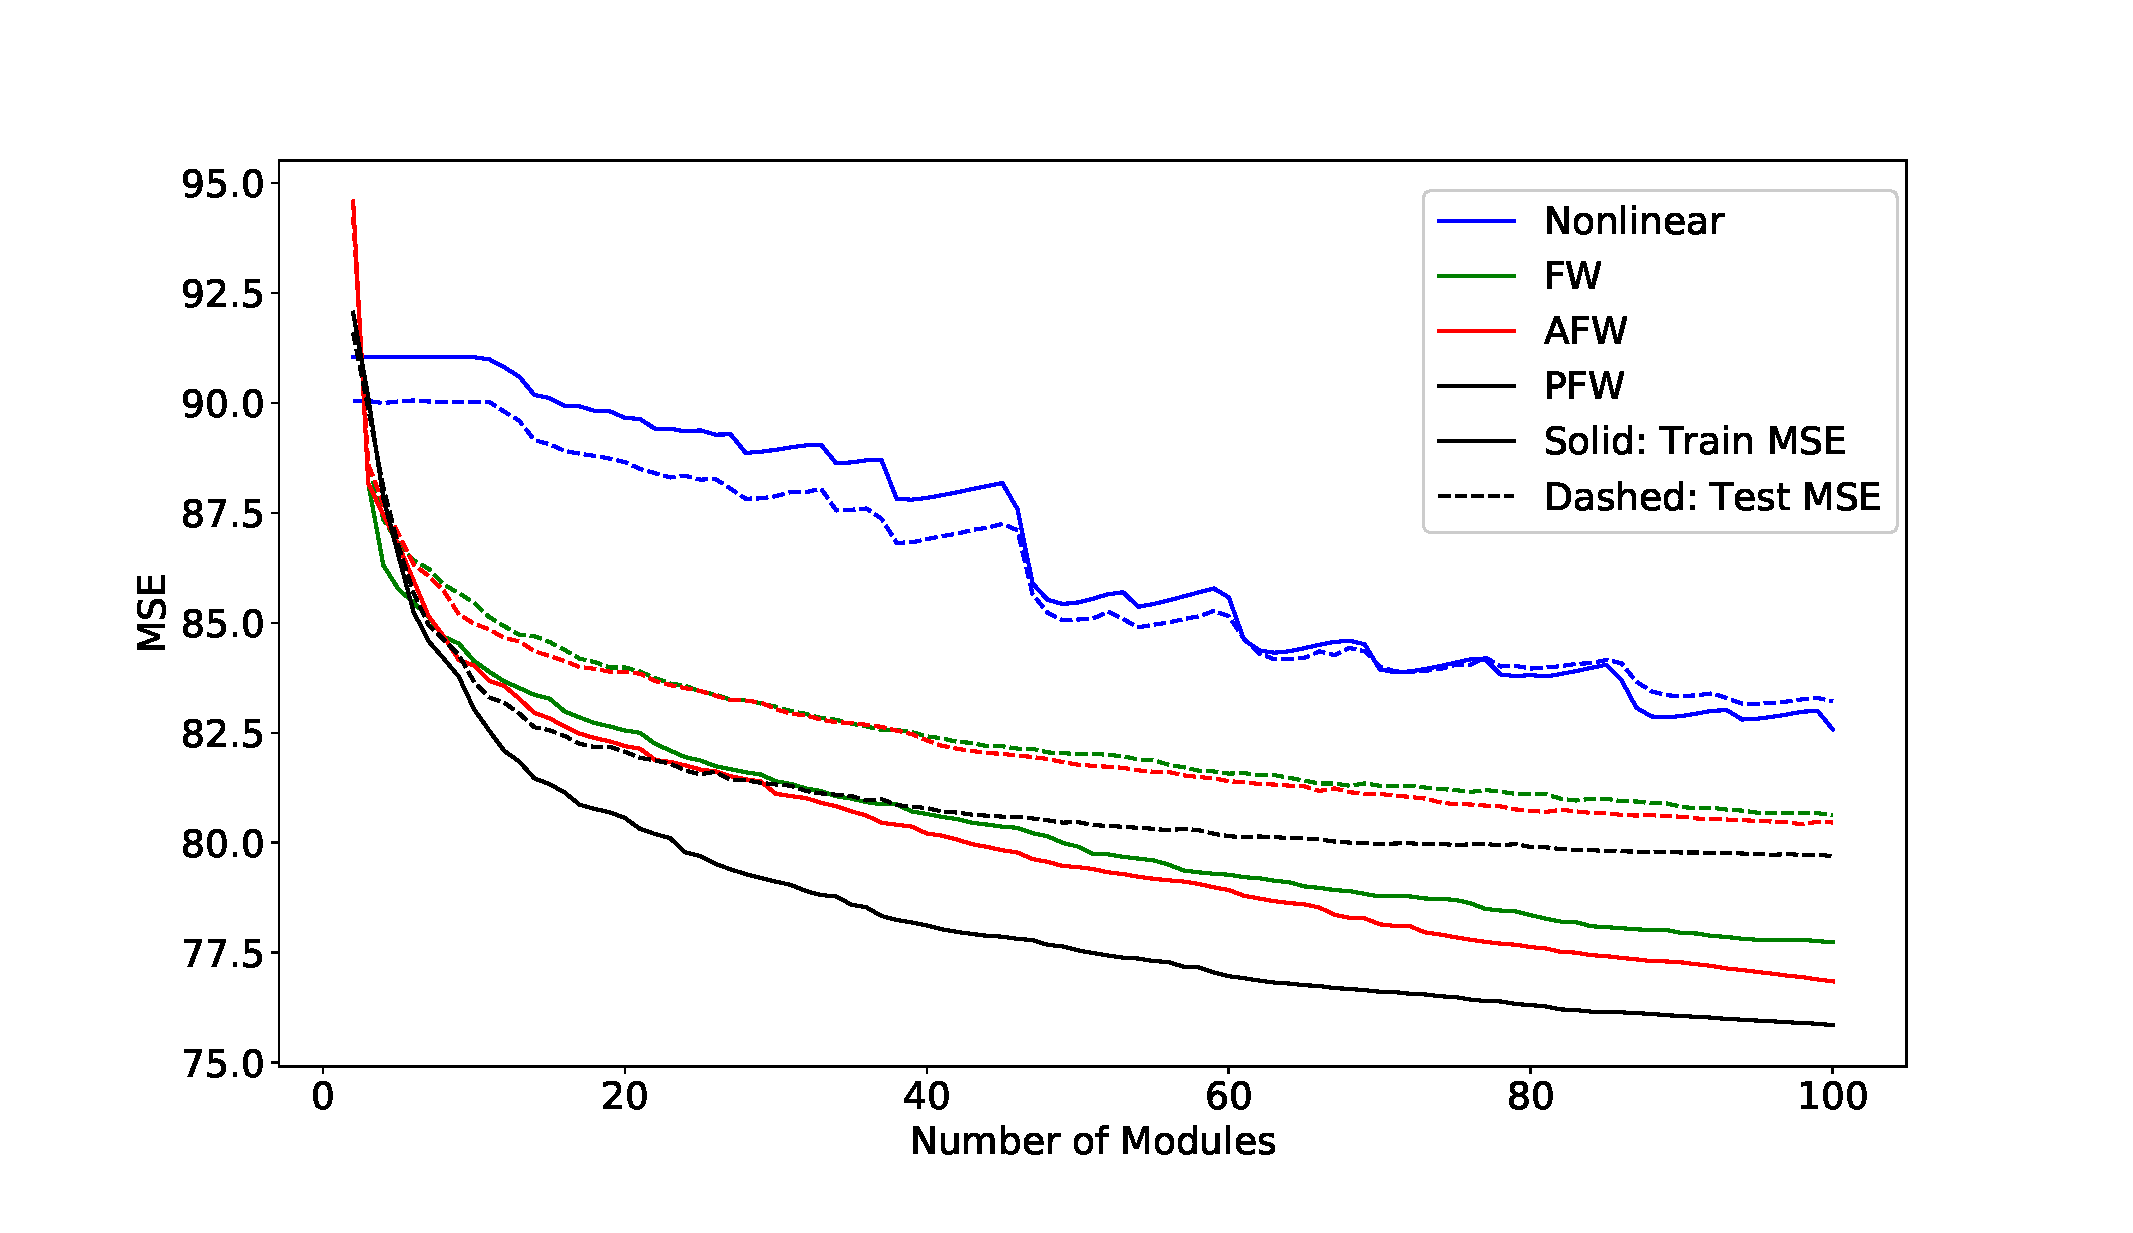
\includegraphics[clip, trim=2cm 1cm 2.5cm 1.5cm, width=\textwidth]{nips_greedy_algs_msd}
\end{minipage}
\begin{minipage}{0.41\textwidth}
\vspace{-1.3ex}
\emph{We empirically compared the above GCE algorithms and found that \emph{PFW is the best in most cases}. The graph shows the training and testing performance of these algorithms on the MSD dataset.}
\end{minipage}

\end{myblock}\vfill

\vspace{-0.2ex}
\begin{myblock}{Empirical Comparison of GCE with Competing Methods}

\begin{minipage}{0.23\textwidth}
\RaggedRight
\emph{Empirical comparison of GCE with Boosting, Random Forest, and Neural Network on a variety of datasets shows that GCE is competitive in the majority of cases.}
\end{minipage}
\begin{minipage}{0.76\textwidth}
\small{
\begin{table}[H]
\centering
\begin{tabular}[t]{lrrrrrrrr} 
\toprule
\textbf{Datasets} & \#\textbf{Samples} & \textbf{GCE} & \textbf{XGBoost} & \textbf{RForest} & \textbf{NN} & \textbf{ConvNet} \\
\midrule
diabetes & 442 & \textbf{42.706} & 46.569 & 49.519 & 43.283 & 44.703 \\
boston & 506 & \textbf{2.165} & 2.271 & 2.705 & 2.217 & 2.232 \\
ca\_housing &20,640& 0.435 & \textbf{0.393} & 0.416 & 0.440 & 0.437  \\
msd & 515,345& \textbf{6.084} & 6.291 & 6.462 & 6.186 & 7.610 \\
\midrule
iris & 150 & \textbf{0.00} & 6.67 & 6.67 & 3.33 & 10.00  \\
wine & 178 & \textbf{0.00} & 2.78 & 2.78 & \textbf{0.0} & \textbf{0.0}  \\
breast\_cancer & 569 & \textbf{3.51} & 4.39 & 8.77 & 3.51 & 4.39 \\
digits & 1,797 & 2.78 & 3.06 & \textbf{2.50} & 3.33 & 3.06 \\
cifar10\_f & 60,000 & \textbf{4.86} & 5.40 & 5.16 & 5.00 & 4.92 \\
mnist & 70,000 & 1.22 & 1.66 & 2.32 & 1.24 & \textbf{1.11} \\
covertype & 581,012 & 26.70 & 26.39 & 27.73 & 26.89 & \textbf{26.56} \\
kddcup99 & 4,898,431 & \textbf{0.01} & \textbf{0.01} & \textbf{0.01} & \textbf{0.01} & \textbf{0.01}\\
\bottomrule
\end{tabular}
\end{table}
}
\end{minipage}

\end{myblock}\vfill

\vspace{-0.2ex}
\begin{myblock}{References}
\vspace{-0.8ex}
\footnotesize{
[1] A. R. Barron. Universal approximation bounds for superpositions of a sigmoidal function. IEEE ToIT, 1993.

[2] Y. Makovoz. Random approximants and neural networks. Journal of Approximation Theory, 1996.

[3] M. Anthony and P. L. Bartlett. Neural network learning: Theoretical foundations. Cambridge University Press, 2009.

[4] S. Mendelson. A few notes on statistical learning theory. Advanced lectures on machine learning, p1-40. Springer, 2003.

[5] S. Mannor, R. Meir, T. Zhang. Greedy algorithms for classification - consistency, convergence, adaptivity. JMLR, 2003.

[6] T. Zhang. Sequential greedy approximation for certain convex optimization problems. IEEE ToIT, 2003.

[7] M. Jaggi. Revisiting Frank-Wolfe: Projection-free sparse convex optimization. ICML, 2013.

[8] S. Lacoste-Julien and M. Jaggi. On the global linear convergence of Frank-Wolfe optimization variants. NIPS, 2015.
}
%\bibliographystyle{abbrv}
%\bibliography{./ref}
\end{myblock}\vfill


}\end{minipage}\end{beamercolorbox}
\end{column}

\end{columns}
\end{frame}
\end{document}
